%% CHAPTER 2 (probably)
%% MODELLING and DATA

\chapter{Modelling and Data} %with GEOS-Chem} % Main chapter title
\label{Model} %better reference name?
  \subsection{List of runs and outputs used in my work TODO: good place for this?}
    TODO: Go through work process and clarify these items
    
    \begin{enumerate}
      \item UCX 
      \begin{enumerate}
        \item Satellite output (1300-1400LT)
        \item Create shape factors for AMF recalculation in OMI
      \end{enumerate}
      
      \item Tropchem (standard)
      \begin{enumerate}
        \item satellite output, daily tracer averages
        \item Recreate the AMFs for OMI when running code from Dr. Paul Palmer, modified by Dr. Luke Surl.
        \item Combined with an identical run where isoprene emissions are halved in order to determine smearing.
        \item TODO: Compare total yearly isoprene emissions before and after new estimate.
      \end{enumerate}
    
      \item Tropchem(isoprene emissions halved)
      \begin{enumerate}
        \item Satellite output used to determine smearing.
      \end{enumerate}
    
      \item Tropchem(biogenic emissions only, all other inventories turned off)
      \begin{enumerate}
        \item Satellite output, hourly biogenic emissions from MEGAN
        \item Used to determine yield for new emissions estimates
        \item TODO: compared to run with updated emissions
      \end{enumerate}
    \end{enumerate}
    NB: for non-UCX runs, satellite output was modified to include tropopause height
  
  \subsection{Reading GEOS-Chem output}
    
    \subsubsection{HEMCO diagnostics}
      
      % Local time offsets
      In order to get hourly MEGAN modelled isoprene emissions, HEMCO (the module of GEOS-Chem dealing with emissions inventories) diagnostic output was created.
      When working with globally gridded data, handling local time offsets becomes more important.
      The hourly output emissions of isoprene is saved using GMT, which needs to be offset based on longitude in order to retrieve local time.
      I do this by setting up a latitude by longitude array which matches the horizontal resolution of the data, filling each gridbox with it's local time offset.
      This offset is determined as one hour per 15 degrees (since 360 degrees is 24 hours), and then used to retrieve global data at any specific local time.
      The retrieval of a daily local time global array is done by index matching the GMT+LT (modulo 24) with the desired hour on this grid over the 24 GMT hours.
    
%%----------------------------------------------------------------------------------------
%%	SECTION
%%----------------------------------------------------------------------------------------
\section{GEOS-Chem}
  \label{Model:GC}
  GEOS-Chem is an atomspheric chemical model (ACM), using a 3-D grid of boxes with transport driven by the GEOS meteorological model and chemistry calculated in each box independently. 
  Many of these terms are described in Section \ref{LR:Models:frames}.



  \subsection{GEOS-Chem isoprene mechanisms}
  \label{Model:GC:Isop}
    \subsubsection{Outline}
      The isoprene reactions simulated by GEOS-Chem were originally based on \cite{Horowitz1998}.
      This involved simulating NO$_X$, O$_3$, and NMHC chemistry in the troposphere at continental scale in three dimensions, with detailed NMHC chemistry with isoprene reactions and products.
      The mechanism was subsequently updated by \citet{Mao2013}, who change the isoprene nitrates yields and add products based on current understanding as laid out in \citet{Paulot2009a,Paulot2009b}.
      Further mechanistic properties, like isomerisation rates, are based on results from four publications: cite{Crounse2011,Crounse2012,Peeters2010,Peeters2011}.
      (TODO: check abstracts Peeters papers).
      \cite{Crounse2011} examines the isomerisations associated with the oxidation of isoprene to six different isomers (ISO$_2$) formed in the presence of oxygen: isoprene $ + OH \rightarrow^{O_2} $ ISO$_2$.
      They determine rates and uncertainties involved in these reactions, and study the rate of formation of C$_5$-hydroperoxyaldehydes (HPALDs) by isomerisation.
      \cite{Crounse2012} examine the fate of methacrolein (MACR), one of the products of isoprene oxidation. 
      Prior to this work MACR oxidation chamber studies were performed in high NO or HO$_2$ concentrations, giving peroxy lifetimes of less than 0.1~s.
      In most environments this is not the case, and MACR products over various NO concentrations and peroxy radical lifetimes are determined in their work.
      \cite{Peeters2010} examine photolysis of hydroperoxy-methyl-butenals (HPALDs, produced by isoprene isomerisation), which regenerates OH levels in areas with high isoprene emissions.
      Additionally, photolysis of photolabile peroxy-acid-aldehydes creates OH and improved model aggreement with continental observations.
      The OH and HPALD interactions are central to maintaining the OH levels in pristine and moderately polluted environments, which makes isoprene both a source and a sink of OH TODO: cite and DL;\url{http://www.nature.com/ngeo/journal/v5/n3/full/ngeo1405.html}.
      
      Formation of isoprene nitrates have an effect on ozone levels through NO$_X$ sequestration, and the yields and destinies of these nitrates is analysed in \citet{Paulot2009a}. 
      They use anion chemical ionization mass spectrometry (CIMS) to determine products of isoprene photooxidation.
      In a chamber with clean air and high NO concentrations, isoprene photooxidation is initially driven by OH addition, followed by NO$_X$ chemistry (150~min - 600~min), and finally HO$_X$ dominated chemistry.
      The yields of various positional isomers of isoprene nitrates is estimated, and pathways of their oxidation products is shown and used in the GEOS-Chem isoprene mechanism \citep{Paulot2009a,Mao2013}. 
      
      In low NO$_X$ conditions, isoprene oxidises to yield 70\% hydroxyhydroperoxides (ISOPOOH), which then oxidises to create dihydroxyperoxides (IEPOX) with OH recycling maintaining the OH levels in the atmosphere \citep{Paulot2009b}.
      In older models isoprene produced ISOPOOH which then titrated OH, however, the loss of OH has not been seen in measurements \citep{Paulot2009b,Mao2013}.
      The isoprene mechanism in GEOS-Chem has been updated to include OH regeneration from oxidation of epoxydiols and slow isomerisation of ISOPO$_2$ \citep{Mao2013}.
      
      ISOPN can be oxidised (by OH) to form nitrated organic products \citep{Paulot2009a}.
      In low NO$_X$ ISOPOO reacts with HO$_2$ (producing hydroxy hydroperoxides, ISOPOOH), RO$_2$ (producing mainly MACR, MVK, and HCHO), or isomerises (1,5-H shift producing MACR, MVK, HCHO, or 1,6-H shift producing hydroperoxyenals HPALDs). 
      ISOPOOH can be oxidised (by OH) to produce epoxydiols (IEPOX), precursors to SOA \citep{Paulot2009b}. 
      HPALDs can photolyse to regenrate OH and small VOCs \citep{Crounse2011,Wolfe2012, Peeters2014} TODO: Check out crounse2011.
      See section \ref{LR:IsopAndVOCs:IsopCascade} for more information.
      
      Under high NO$_X$ conditions, isoprene undergoes OH addition at the 1 and 4 positions, becoming $\beta$ (71\%) or $\delta$ (29\%) hydroxyl peroxy radicals (ISOPO$_2$). 
      The $\beta$-hydroxyl reacts with NO$_X$ and produces HCHO (66\%), methylvinylketone (40\%) (MVK), methacrolein (26\%), and $\beta$-hydroxyl nitrates (6.7\%) (ISOPNB).
      The $\delta$-hydroxyl reacts with NO to form $\delta$-hydroxyl nitrates (24\%) (ISOPND), and ISOPNB (6.7\%).
      ISOPNB and ISOPND yield first generation isoprene at 4.7\% and 7\% respectively.
      
      Under low NO$_X$ conditions, ISOPO$_2$ may react with HO$_2$ to form ISOPOOH.
      In this case there is also production of HCHO (4.7\%), MVK(7.3\%), and MACR (12\%).
      As stated in earlier; most ISOPOOH will form IEPOX (epoxydiols) after reacting with OH and lead to OH regeneration.
      The other mechanism in low NO$_X$ environments is unimolecular isomerisation of ISOPO$_2$.
      This leads to production of hydroperoxyaldehydes (HPALDS), which generally photolyse and have an OH yield of 100\%.
      \citet{Mao2013} show that a lower (factor of 50) rate constant for ISOPO$_2$ isomerisation leads to better organic nitrate aggreements with ICARTT. 
      
      This update leads to more accurate modelling of OH concentrations, especially in low NO$_X$ conditions common in remote forests.
      Prior to \citet{Mao2012}, measurements of OH in high VOC regions may have been up to double the real atmospheric OH levels, due to formation of OH inside the instrument.
      \citet{Mao2012} examine an upgraded method of measurement, and compare these against a regional atmospheric chemistry model (RACM2), with the OH recycling updates from \citet{Paulot2009b} as discussed in prior paragraphs.
      
      The updates to isoprene chemistry by \citet{Mao2013}, and those shown in \cite{Crounse2011,Crounse2012} are the last before version 11, which was not used in this work.
      
      The full current mechanism is described online at \url{http://wiki.seas.harvard.edu/geos-chem/index.php/New_isoprene_scheme}.

    \subsubsection{Emissions from MEGAN}
      \label{Model:GC:Isop:MEGAN}
      MEGAN simulates biogenic emissions of various gases including isoprene, based on various meteorological, land cover, and plant type parameterisations.
      
      One of the important parameters in Australia is the soil moisture activity factor($\gamma_{SM}$), which can have large regional affects on the isoprene emissions \citep{Sindelarova2014,Bauwens2016}.
      Generally if soil moisture is too low, isoprene emissions stop \citep{Pegoraro2004,Niinemets2010}, however in many Australian regions the plants may be more adapted to lower moisture levels. (TODO: Find cites for this - talk from K Emerson at Stanley indicated this)
      GEOS-Chem runs MEGANv2.1, which has three possible states for isoprene emissions based on the soil moisture ($\theta$):
      \begin{align*}
        \gamma_\mathrm{SM} & = 1 && \theta > \theta_1 \\
        \gamma_\mathrm{SM} & = (\theta-\theta_w)/\Delta\theta_1  && \theta_w < \theta < \theta_1 \\
        \gamma_\mathrm{SM} & = 0 && \theta < \theta_w \\
      \end{align*}
      where $\theta_w$ is the wilting point, and $\theta_1$ determines when plants are near the wilting point.
      The wilting point is set by a land based database from \citet{Chen2001}, while $\theta_1$ is set globally based on \citet{Pegoraro2004}.
      
      In GEOS-Chem the isoprene emissions can be globally multiplied by a constant factor.
      By running the model two extra times, with the biogenic isoprene emissions turned off in one run and halved in another, while other parameters remain unchanged. 
      These modified runs allow an estimate of model sensitivity to isoprene emissions and smearing impact as described in Section \ref{BioIsop:Methods:Smearing}.
        
  \subsection{Running GEOS-Chem (before isop?)}
  \label{Model:GC_running}
    \subsubsection{Installation and requirements}
      GEOS-Chem instructions for download, compilation, and running can be found in the user guide provided by Harvard: \url{http://acmg.seas.harvard.edu/geos/doc/man/}.
      In order to build and run GEOS-Chem a high-speed computing system is optimal, as globally gridded chemical calculations can take a long time to perform.
      I installed GEOS-Chem onto a suitably configured workspace on the National Computational Infrastructure (NCI, \url{http://nci.org.au/}). 
      This workspace included access to compilers and libraries which are needed to build the Fortran based GEOS-Chem source code, and IDL, Python, and various editors and scripting languages to read, run, edit, and analyse both GEOS-Chem and its output.
        
      After downloading GEOS-Chem, the code can be compiled with different options for resolution and chemical mechanisms.
    \subsubsection{Options}
    
    \subsubsection{Tropchem mechanisms}
    
    \subsubsection{UCX mechanisms}
    % TODO: layout reasons why isoprene differs between runs
    %    In GeosCore/fast_jx_mod.F:
    %      strat aerosols are scaled somehow at line 2922, looks like it affects SSA.
    %      line 4138: comment says ozone calculated online.
    %	  TOMS/SBUV O3 are read by toms_mod.f, passed to FAST-J routine ``set_prof.f''. in UCX the stratospheric O3 is calculated online
    %    In GeosCore/calcrate.F:
    %      line 1489 comment says rates are limited to prevent solver failure
    %	if lifetime of A is below PSCMINLIFE, limit reaction rate to yield the specified lifetimedepletion
    %      Line 1724
    %        ! SPECIAL TREATMENT FOR O3+hv -> OH+OH (trop-only simulation)
    %        !                    or O3+hv -> O+O2  (UCX simulation)
    %      line 1752:
    %      #if defined( UCX )
    %        IF ( NKO3PPHOT(NCS) > 0 ) THEN
    %          PHOTVAL_2 = NKO3PPHOT(NCS) - NRATES(NCS)
    %          NKN_2     = NKNPHOTRT(PHOTVAL_2,NCS)
    %        ENDIF
    %      #endif
    %      line 1771:
    %        comment: change rate of O(1D) + N2 to 3.1e-11 at 298K (from 2.6e-11)...
    %        if not defined UCX:
    %	  RO1Dp1H2O, RO1Dp1H2, RO1D, (and maybe 2 RRates) are changed.
    
    \subsection{Run comparisons}
    
      There are many options available when running GEOS-Chem depending on the desired chemistry, resolution, meteorology, and boundary conditions.
      Here we compare the model output with and without enabling the Universal tropospheric-stratospheric Chemistry eXtension (UCX).
      %From version 11 of GEOS-Chem, the UCX mechanism is enabled by default.
      Both runs use 2$^{\circ}$ latitude by 2.5$^{\circ}$ longitude, however the UCX mechanism is run with 72 vertical levels from the surface to the top of the atmosphere (TOA$\sim$0.1~hPa), while the standard (tropchem) run uses 47 levels.
      The extra vertical levels are added in the stratosphere, providing finer vertical resolution from around 70~hPa to the top of the atmosphere.
      For both runs the inpup parameters such as MEGAN emissions and GEOS-5 meteorological fields are identical.
      
      GEOS-Chem output of HCHO does not differ much between runs with or without the Unified Chemistry eXchange (UCX).
      Figure \ref{Model:GC_Running:UCXvsTrop_HCHO} shows an example of surface HCHO amounts with and without UCX turned on.
      The differences do not exceed 3\% over Australia for the averaged month of January, 2005.
      
      \begin{figure}%[!htbp] % TODO: remove 'rerun' plot, use normal and delete rerun thingy so it's not confusing later.
        % These figures created in GC_test.py -> TODO:
        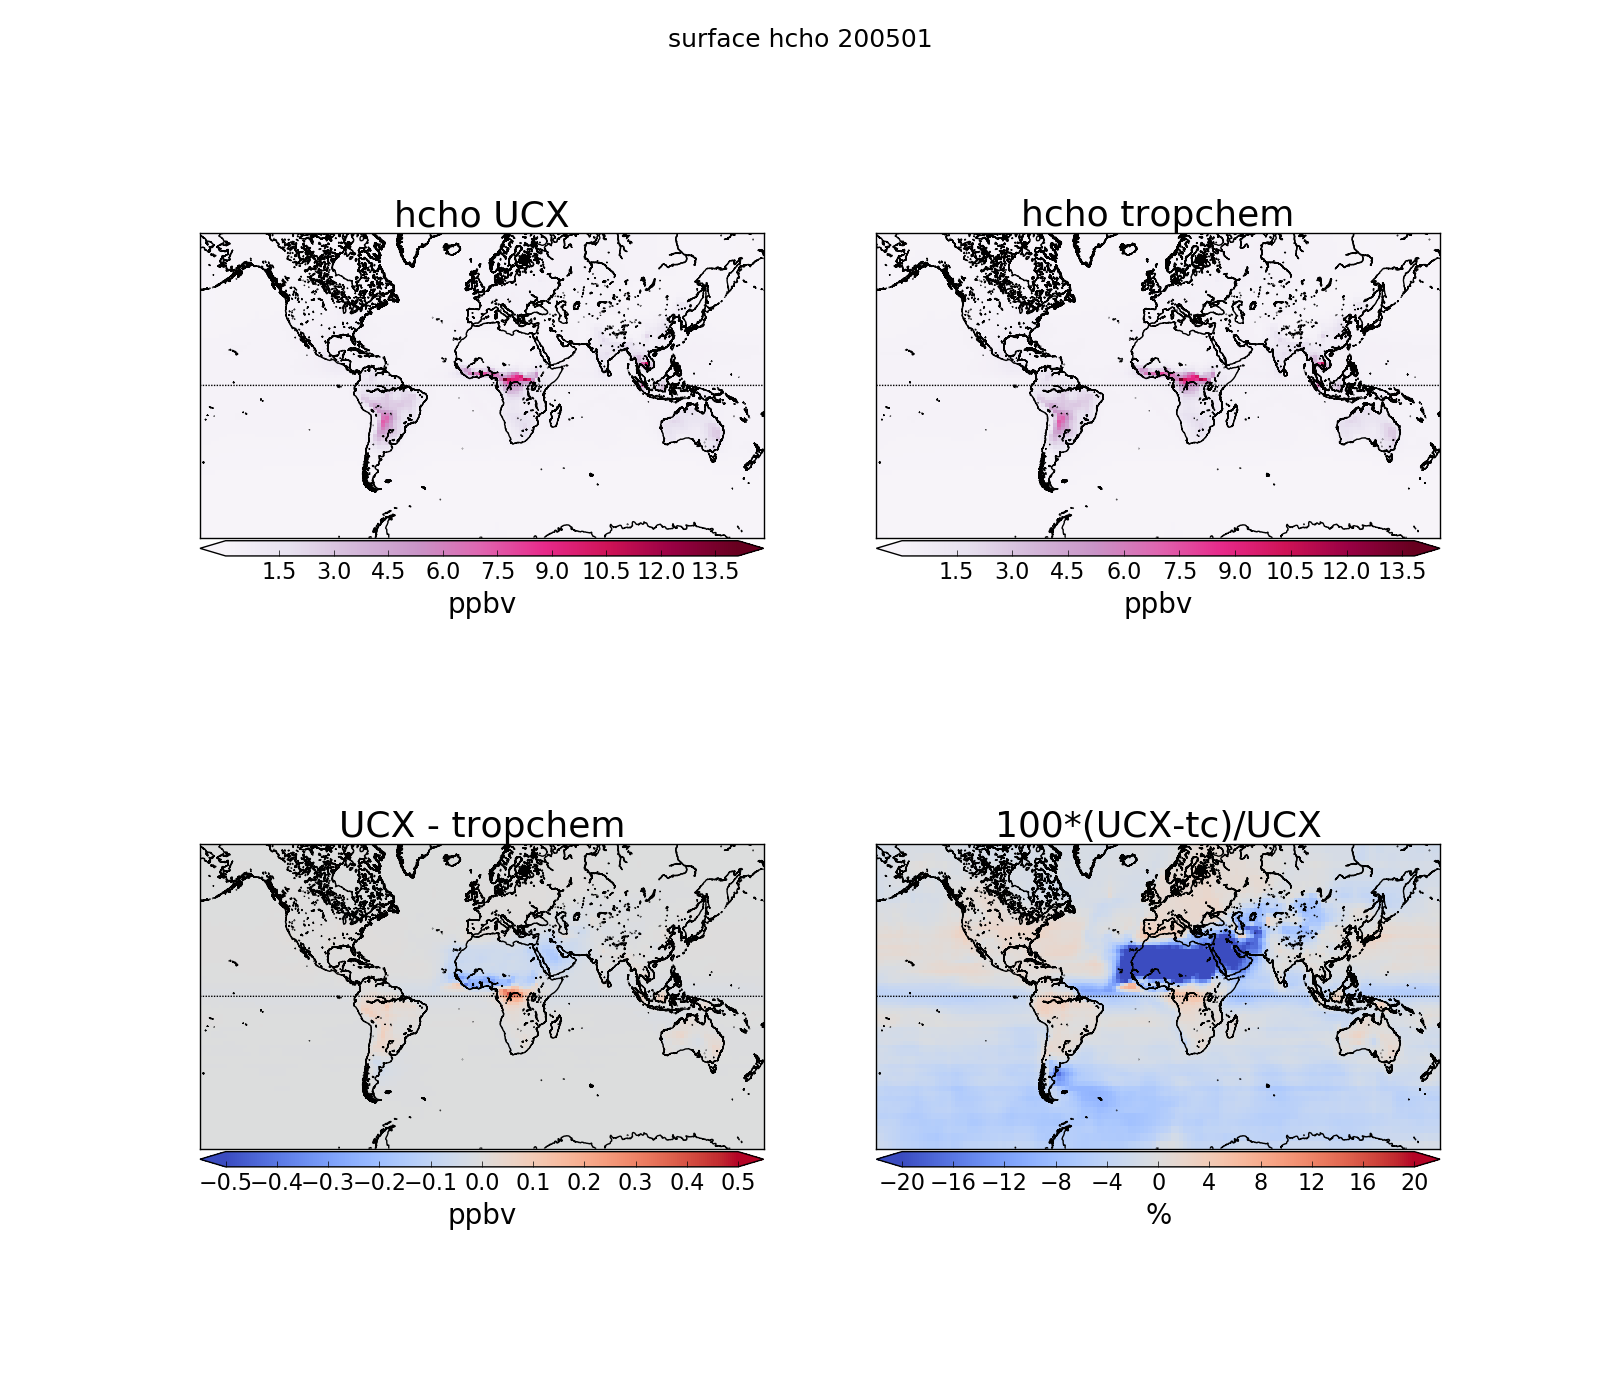
\includegraphics[width=\textwidth]{Figures/HCHO/GClink/UCX_vs_trp_glob_200501_hcho_rerun.png}
        \caption{ %
          Surface HCHO simulated by GEOS-Chem with UCX (top left), and without UCX (top right), along with their absolute and relative differences(bottom left, right respectively).
          Amounts simulated by GEOS-Chem for the 1st of January, 2005.
        }
        \label{Model:GC_Running:UCXvsTrop_HCHO}
      \end{figure}
      
      Figure \ref{Model:GC_Running:UCXvsTrop_Isop} shows the differences in surface isoprene amounts over Australia.
      Here we start to see a higher relative difference in concentrations, although this is generally over the areas with less absolute concentrations. 
      Very little isoprene is seen away from the continent (4-5 orders of magnitude less), due to the short lifetime of isoprene, and lack of emissions over the oceans.
      Generally isoprene is 0-30\% higher over Australia when the UCX mechanism is turned on.
      This enhancement can be seen throughout the entire tropospheric column as shown by Figure \ref{ch_HCHO:fig:isoptropUCXcomparison}.
      \begin{figure}%[!htbp]
        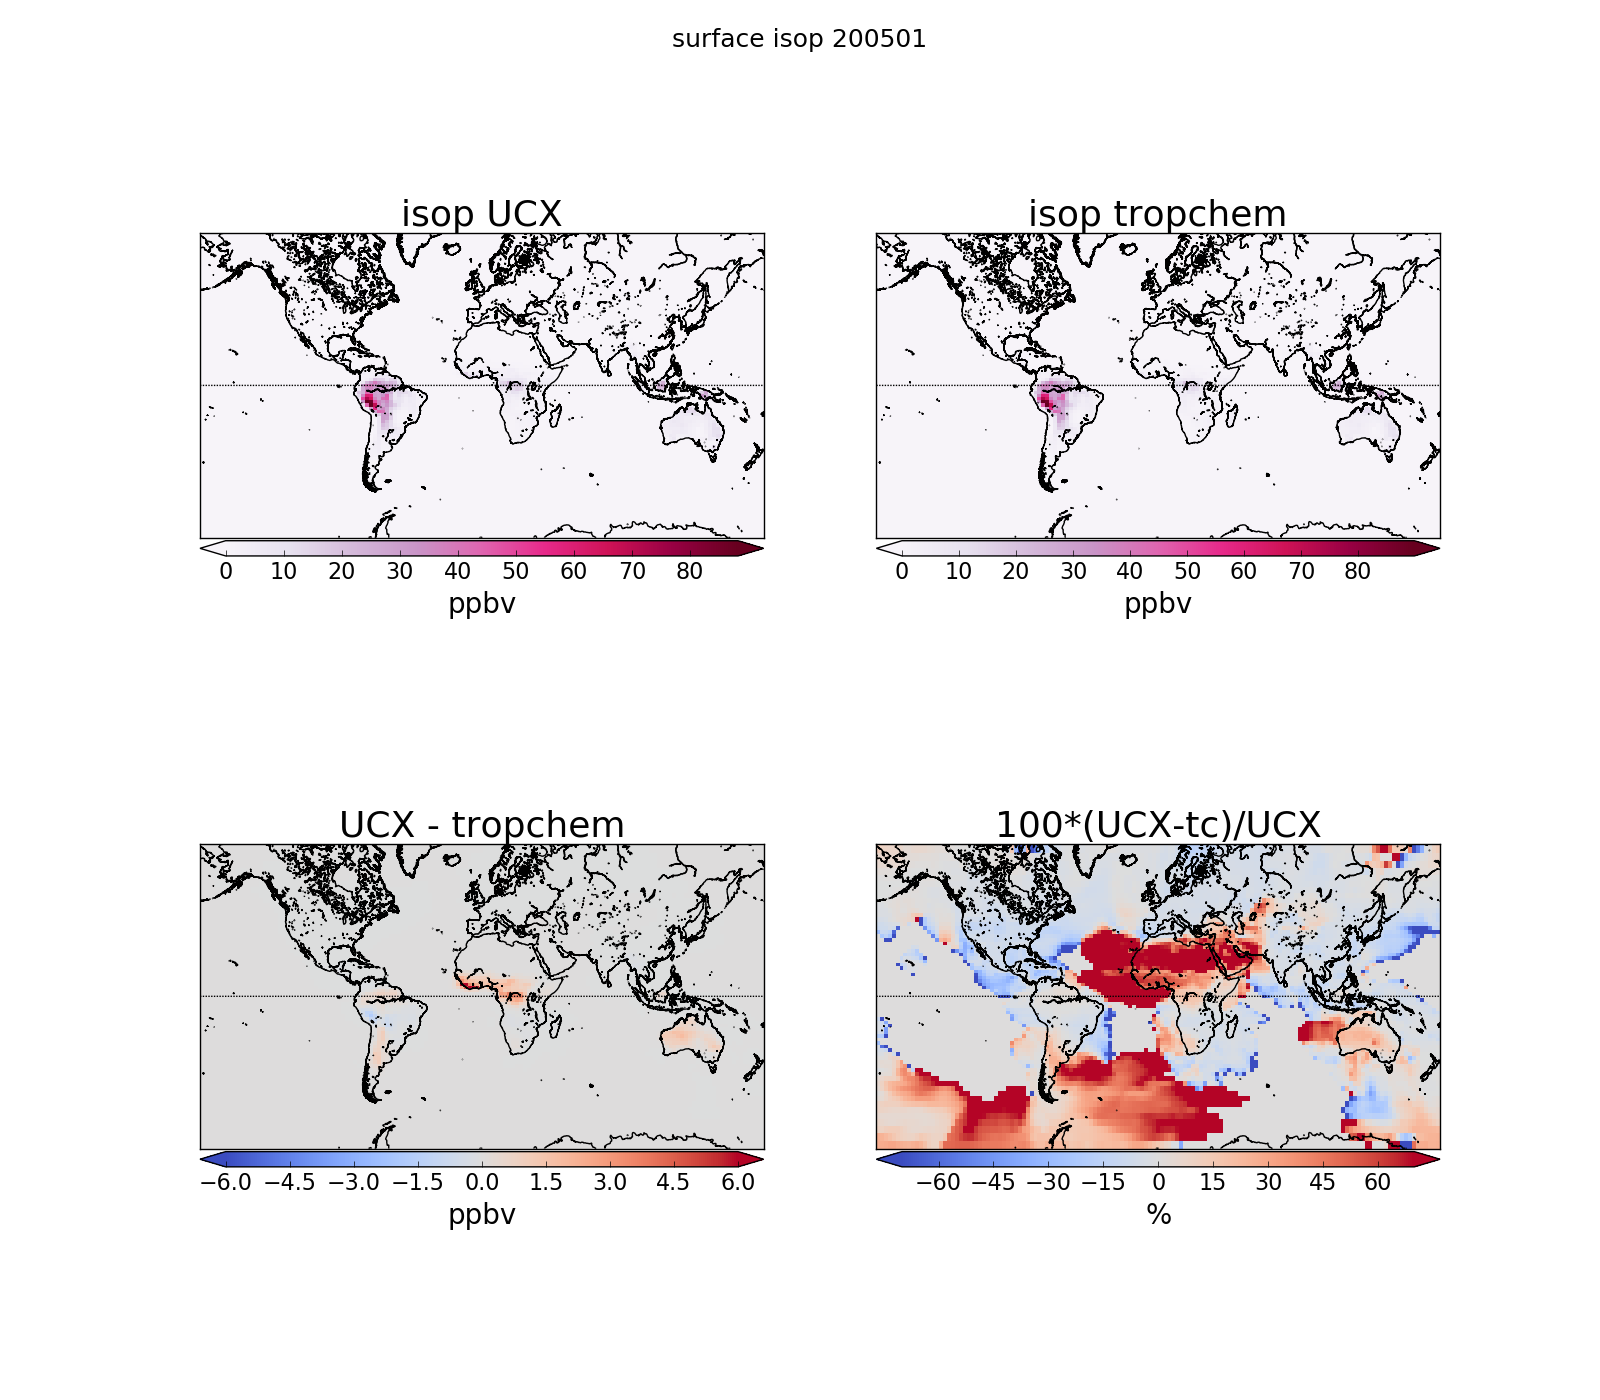
\includegraphics[width=\textwidth]{Figures/HCHO/GClink/UCX_vs_trp_glob_200501_isop_rerun.png}
        \caption{ %
          As figure \ref{Model:GC_Running:UCXvsTrop_HCHO}, except looking at isoprene. 
        }      
        \label{Model:GC_Running:UCXvsTrop_Isop}
      \end{figure}
      
      
      Figure TODO: shows the columns for isoprene and HCHO simulated by our two mechanisms over Australia in January of 2005.
      The differences are minimal compared to other uncertainties in both AMF calculation and emissions estimation.
      
      
      TODO: The difference in isoprene between UCX and tropchem is likely caused by differences in the modelled radiation reaching the troposphere due to differences in simulated ozone in the stratosphere.
      With higher stratospheric ozone levels, less radiation would reach the troposphere, changing the photochemistry.
      Figure \ref{Model:GC_Running:UCXvsTrop_O3} shows the total column ozone between UCX and non-UCX runs, we can see that UCX has TODO: less or more ozone over Australia/USA in January.
          
      \begin{figure}%[!htbp]
        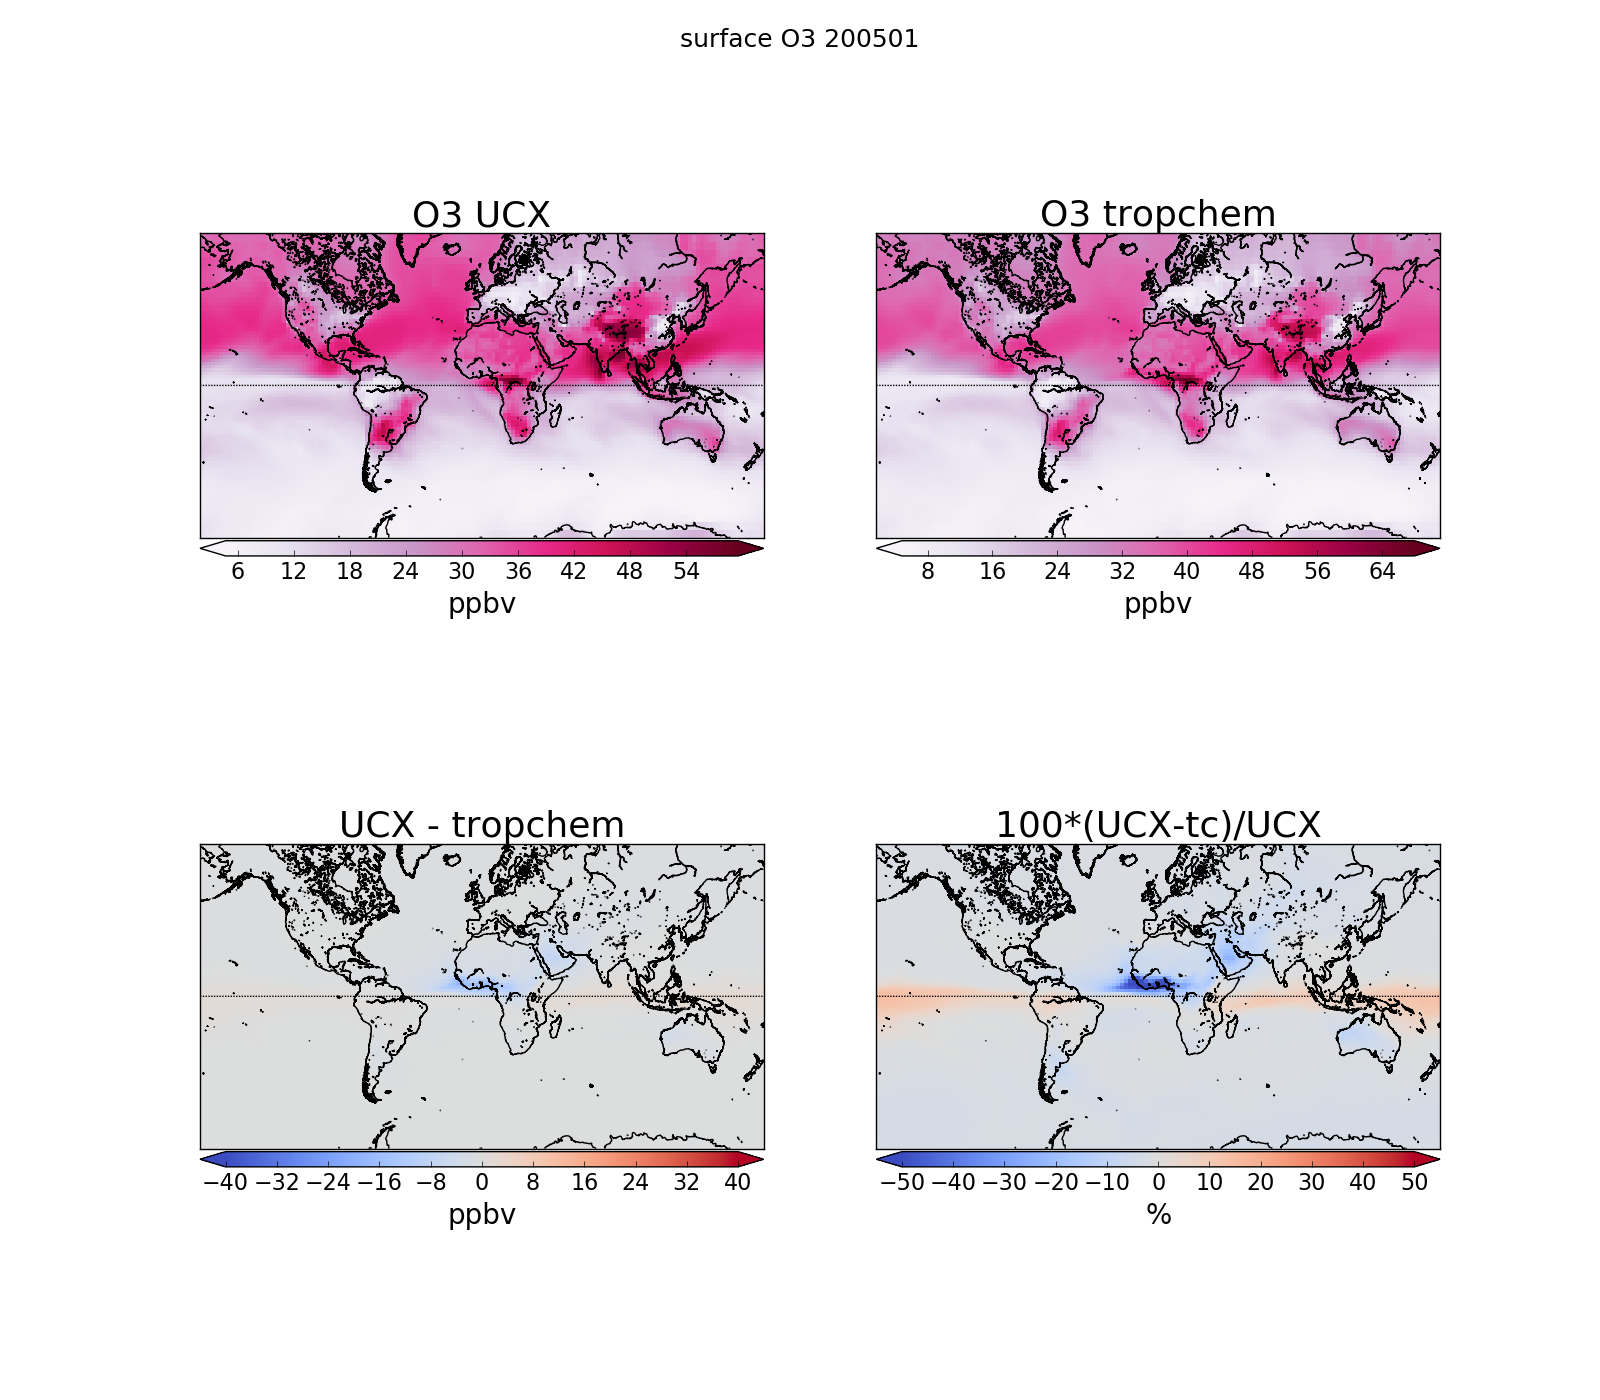
\includegraphics[width=\textwidth]{Figures/HCHO/GClink/UCX_vs_trp_glob_200501_O3_rerun.png}
        \caption{%
          As figure \ref{Model:GC_Running:UCXvsTrop_HCHO}, except looking at ozone. 
        }
        \label{Model:GC_Running:UCXvsTrop_O3}
      \end{figure}

\section{CAABA/MECCA}
\label{Model:CM}


\section{Campaigns and datasets}
  \label{Model:Datasets}
  Here I will describe the various datasets I've used to analyse GEOS-Chem output.
  These datasets are also used to determine how suitable GEOS-Chem is in calculation of isoprene emissions estimations in chapter \ref{BioIsop} and ozone transport extrapolations in chapter \ref{Ozone}.
  
  TODO: these summaries.
  
  %Omi summary
  \subsection{OMI Satellite measurements}
  \label{Model:Datasets:OMI}
  
    \subsubsection{OMI HCHO}
    Recalculated OMI formaldehyde columns are used as a basis for estimating isoprene emissions in Chapter \ref{BioIsop}
    
    HCHO has been found to be biased low in several studies \cite[eg.][]{Zhu2016,DeSmedt2015,Barkley2013}
  
    \subsubsection{OMI NO2}
    \label{Model:Datasets:OMNO2d}

  Daintree summary (P. Nelson)
  
  % TODO: MUMBA summary
  \subsubsection{Marine and Urban MBA ? (MUMBA)}
    \label{Model:Datasets:MUMBA}
  
  \subsubsection{Sydney Particle Studies (SPS1, SPS2)}
    \label{Model:Datasets:SPS}
    Two VOC and other trace gas measurement campaigns took place at the Westmead Air Quality Station scientists from CSIRO, OEH, and ANSTO. 
    Stage 1 (SPS1) was from 5 February to 7 March in 2011, while stage 2 (SPS2) ranged from 16 April to 14 May 2012.
    
    Two instruments measured VOC concentrations: one was a Proton transfer reaction mass spectrometer (PTR-MS), the other a gas chromatographer (GC) with an equipped flame ionisation detector (FID).
    The PTR-MS uses chemical ionisation mass spectrometry and can quantify VOCs at high temporal resolution ($< 1$~s).
    It was calibrated several times per day against hcho, isoprene, $\alpha$-pinene, and several more VOCs. Further details can be found in \cite{Dunne2012,Dunne2017} (TODO: Check papers).
    The output lists hourly averaged ppbv concentrations of trace gases based on the mass to charge ratio (m/z), which for isoprene is 69.
    It's possible that other chemicals (such as Furan, with the same m/z) interfered with this value, especially at low ambient isoprene concentrations and towards the end of autumn (SPS2) when wood fires usage starts to become frequent (TODO cite something).
    The GC-FID analysed samples collected in multi-absorbent tubes, with lower temporal resolution but no interferences. GC-FID data is averaged from 0500-1000~LT, and 1100-1900~LT. Further details for this method can be found in TODO: cite Min et al 2016.
    
    Figure TODO: shows isoprene and formaldehyde over the course of these two campaigns, as well as the detection limits (dashed lines), as measured by PTR-MS. In order to compare with GEOS-Chem output a daily average and an overpass time (1200-1300 LT) average are both created from these data.
    In averaging, any measurements below the machine detection limit are set to half of the detection limit, as done in (TODO: doi:10.5194/acp-15-223-2015, 2015) which should minimise any introduced bias.

\section{Analysing output}
\label{Model:Analysis}
  
  \subsection{Circadian emissions cycle}
    HEMCO diagnostics provide the simulated MEGAN isoprene emissions at high temporal resolution.
    TODO: Figure X shows the daily emissions cycles for a few regions over each season. 
    The regions are labelled in the top panel, and seasonally averaged emissions from grid-boxes in each region are shown below.
    TODO: Figure XX shows the emissions from SPS1 and 2 compared against GEOS-Chem estimates in the same grid square.
    
  \subsection{HCHO: Simulated vs Measured}
  \label{Model:Analysis:HCHO}
    
    HCHO precursors are heavily tied to temperature (TODO:cite), and model output shows how higher temperature leads to an increase in HCHO levels.
    Figures \ref{Model:Analysis:HCHO:fig_hcho_vs_temp_SEA_200501} - \ref{Model:Analysis:HCHO:fig_hcho_vs_temp_SWA_200501} show the relationship between temperature and HCHO, for January 2005, within subsets of Australia.
    A reduced major axis regression is used to determine the linear slopes between surface temperature (X axis) and HCHO (Y axis).
    This gives us a linear regression for each region however it's clear from the straight line and from literature that the relationship is not linear but rather exponential (TODO: cite and example studies).
    Using the natural log of HCHO we can take the linear regression and then exponentiate each side in the equation $\ln{Y} = m{X}+b$ to get ${Y} = \exp{m{X}+b}$. 
    This gives us the exponential fit as shown, with the corellation coefficient between $\ln{HCHO}$ and temperature, which is not directly comparable to the linear coefficient.
    The distributions of exponential corellation coefficients and exponential 'm' terms is shown in the embedded plot, with one datapoint available for each grid square where the regression is performed.
    
    
    \begin{figure}
      \includegraphics[width=\textwidth]{Figures/HCHO/GClink/HCHO_vs_temp_SEA_20050101-20050131.png}
      \caption{%
        Top panel: surface temperature averaged over January 2005.
        Bottom panel: surface temperature correlated against temperature over January 2005, with different colours for each gridbox, and the combined correlation. 
        A reduced major axis regression is used within each gridbox (shown in top panel) using daily overpass time surface temperature and HCHO amounts (ppbv).
        The distribution of slopes and regression corellation coefficients (one datapoint per gridbox) for the exponential regression is shown in the embedded plot.
      }
      \label{Model:Analysis:HCHO:fig_hcho_vs_temp_SEA_200501}
    \end{figure}
    
    \begin{figure}
      \includegraphics[width=\textwidth]{Figures/HCHO/GClink/HCHO_vs_temp_NA_20050101-20050131.png}
      \caption{%
        As figure \ref{Model:Analysis:HCHO:fig_hcho_vs_temp_SEA_200501} but for northern Australia.
      }
      \label{Model:Analysis:HCHO:fig_hcho_vs_temp_NA_200501}
    \end{figure}
    
    \begin{figure}
      \includegraphics[width=\textwidth]{Figures/HCHO/GClink/HCHO_vs_temp_SWA_20050101-20050131.png}
      \caption{%
        As figure \ref{Model:Analysis:HCHO:fig_hcho_vs_temp_SEA_200501} but for south-western Australia.
      }
      \label{Model:Analysis:HCHO:fig_hcho_vs_temp_SWA_200501}
    \end{figure}
    
  \subsection{Accounting for Fires}
  
    TODO: look at yearly corellation, compare to exponential curve and look for fire outliers
    As seen in TODO: citation, HCHO concentrations scale exponentially with temperature.
    This allows another method for detecting the influence of non-biogenic HCHO emission/creation by looking for outliers above the curve at low temperature.
    \cite{Zhu2013_poster} has a similar analysis over south-eastern USA showing an exponential correlation of ${HCHO} = \exp(0.15*{T}-9.07)$.
    
    In GEOS-Chem we can simply turn off pyrogenic emissions, however in satellite datasets we need to mask the fires using MODIS fire counts.
    
    
  \subsection{Accounting for NOx}
  \label{Model:Analysis:NOx}
    
    NO$_X$ concentrations affect HCHO yield, isoprene lifetimes, and other things due to affects on the atmospheres oxidative capacity.
    This means that if the model is poorly simulating NO$_X$, the yield (and transport, see \ref{BioIsop:Methods:Smearing}) may be poorly estimated.
    
    Simulated GEOS-Chem tropospheric NO$_2$ columns averaged from 1300-1400~LT are compared against OMNO2d data (Sec. \ref{Model:Datasets:OMNO2d}). 
    Figure \ref{Model:Analysis:NOx:fig_GC_vs_OMNO2d_2005} shows the direct comparison between these datasets averaged over the month of January, 2005.
    It's clear that the OMNO2d product can pick out Sydney and Melbourne as NO$_2$ hotspots, which are underestimated by GEOS-Chem due to averaging over the 2x2.5\degr horizontal resolution.
    Over much of the country GEOS-Chem overestimates NO$_2$ by 10-60\%, except in NA and northern Queensland where up to 50\% underestimation occurs.
    
    \begin{figure}[!htbp]
      % Figure from GC_tests.py GC_vs_OMNO2d, then modified in paint
      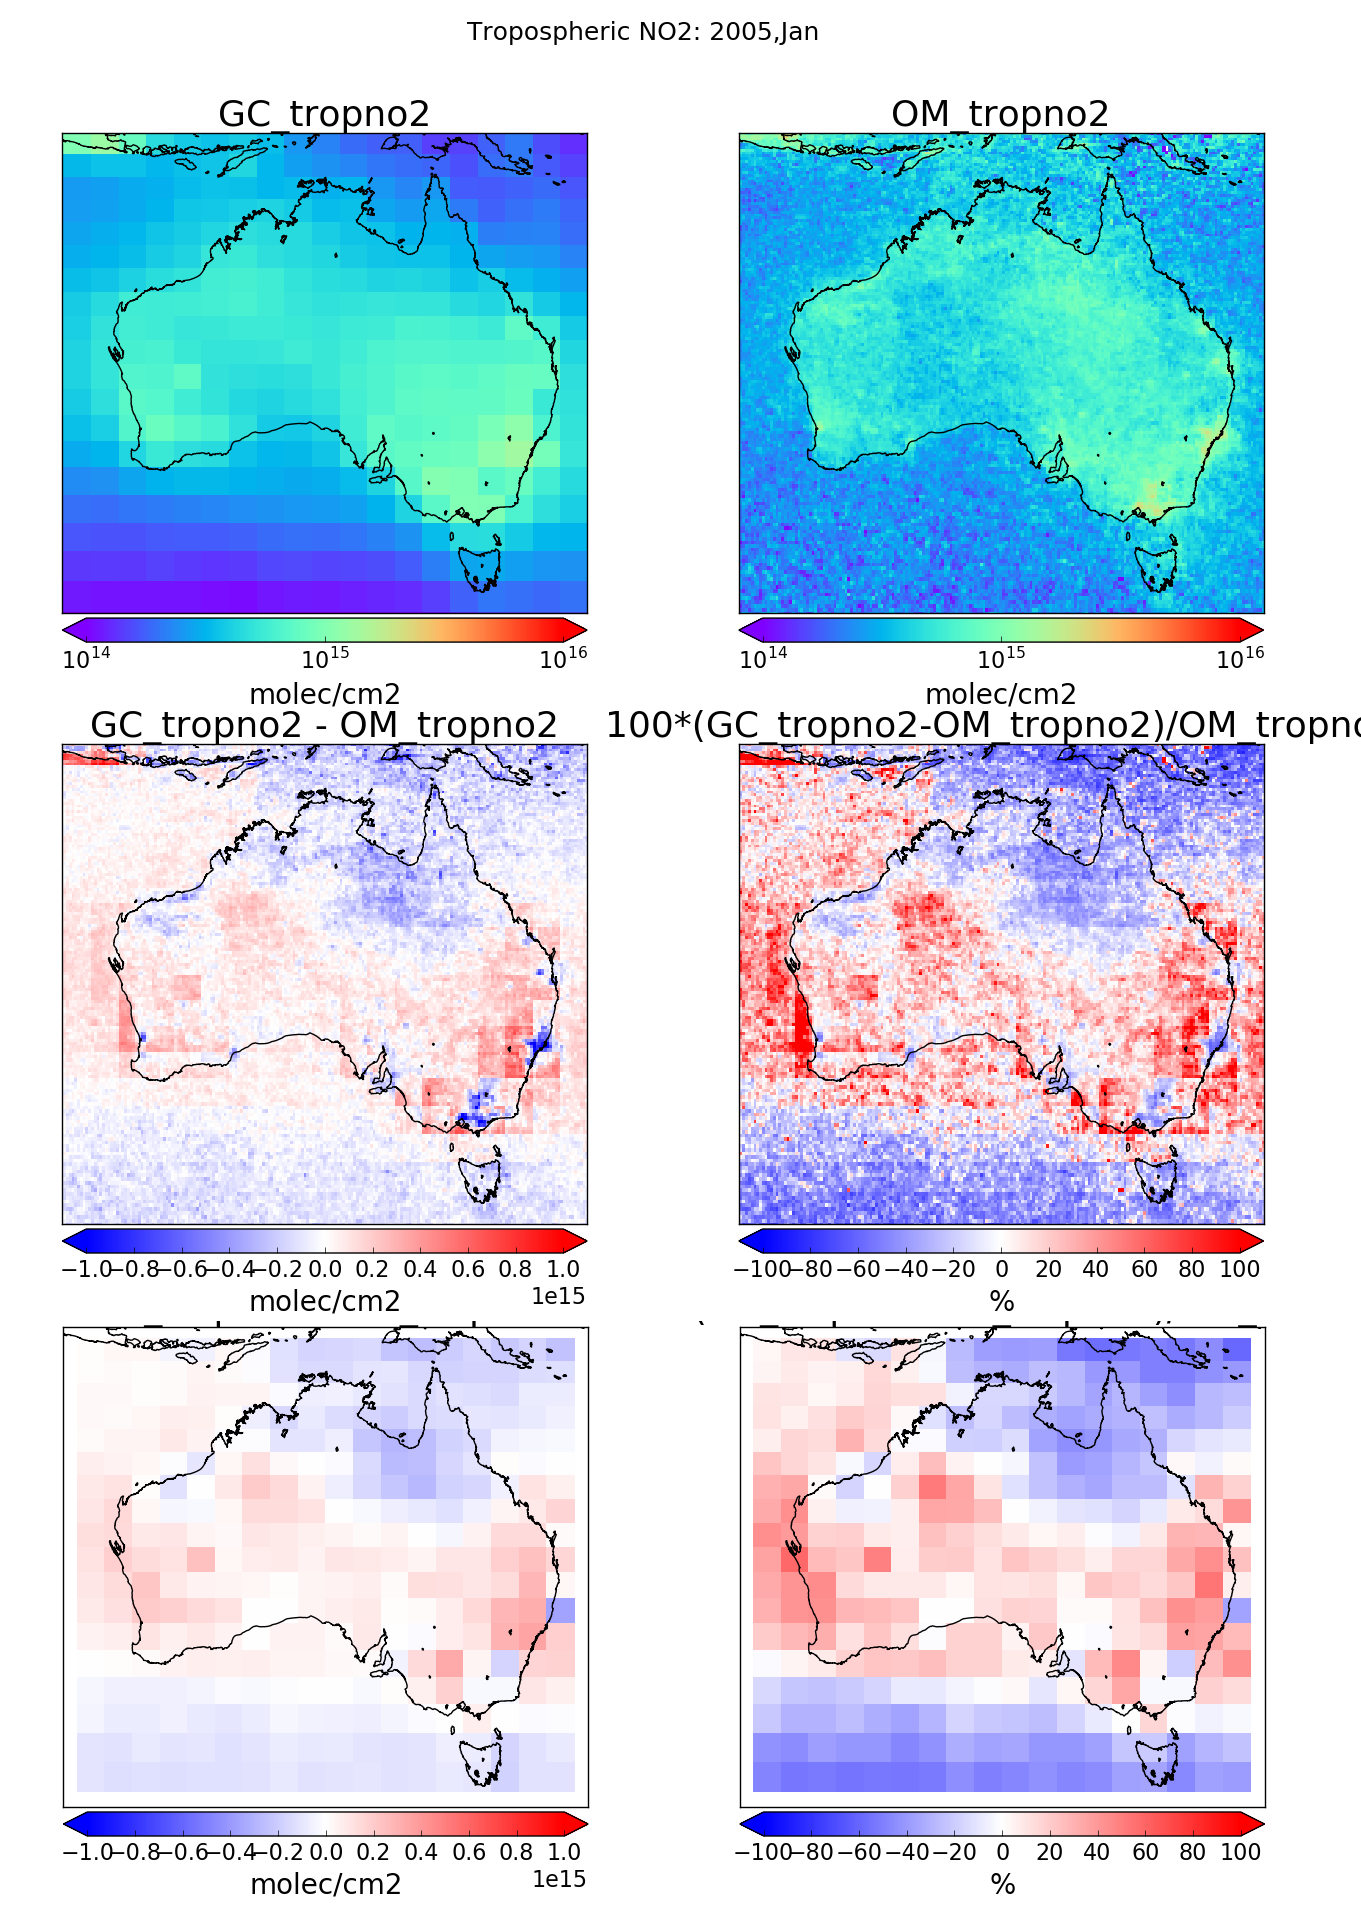
\includegraphics[width=\textwidth]{Figures/GEOSChem/GC_vs_OMNO2_bires_200501.png}
      \caption{%
        Row 1 shows the tropospheric columns in molec cm$^{-2}$.
        Row 2 shows the absolute and relative differences with GEOS-Chem mapped onto the higher resolution of OMNO2d.
        Row 3 shows the differences with OMNO2d columns averaged into the lower resolution of GEOS-Chem.
      }
      \label{Model:Analysis:NOx:fig_GC_vs_OMNO2d_2005}
    \end{figure}
    
  \subsection{HCHO Comparisons}
    TODO: GOME2 HCHO stuff?
    During days with more than one HCHO column measurement we can more confidently fit the cycle. 
    For example EOS AURA's OMI measurements from 2004 can be combined with MetOp-A's GOME2 after October 2006, with daily overpasses by OMI and GOME2 at 1345 and 0930 respectively.